\documentclass[]{article}
\usepackage{lmodern}
\usepackage{amssymb,amsmath}
\usepackage{ifxetex,ifluatex}
\usepackage{fixltx2e} % provides \textsubscript
\ifnum 0\ifxetex 1\fi\ifluatex 1\fi=0 % if pdftex
  \usepackage[T1]{fontenc}
  \usepackage[utf8]{inputenc}
\else % if luatex or xelatex
  \ifxetex
    \usepackage{mathspec}
  \else
    \usepackage{fontspec}
  \fi
  \defaultfontfeatures{Ligatures=TeX,Scale=MatchLowercase}
  \newcommand{\euro}{€}
\fi
% use upquote if available, for straight quotes in verbatim environments
\IfFileExists{upquote.sty}{\usepackage{upquote}}{}
% use microtype if available
\IfFileExists{microtype.sty}{%
\usepackage{microtype}
\UseMicrotypeSet[protrusion]{basicmath} % disable protrusion for tt fonts
}{}
\usepackage[margin=1in]{geometry}
\usepackage{hyperref}
\PassOptionsToPackage{usenames,dvipsnames}{color} % color is loaded by hyperref
\hypersetup{unicode=true,
            pdftitle={month\_by\_month},
            pdfauthor={Sarp Uner},
            pdfborder={0 0 0},
            breaklinks=true}
\urlstyle{same}  % don't use monospace font for urls
\usepackage{color}
\usepackage{fancyvrb}
\newcommand{\VerbBar}{|}
\newcommand{\VERB}{\Verb[commandchars=\\\{\}]}
\DefineVerbatimEnvironment{Highlighting}{Verbatim}{commandchars=\\\{\}}
% Add ',fontsize=\small' for more characters per line
\usepackage{framed}
\definecolor{shadecolor}{RGB}{248,248,248}
\newenvironment{Shaded}{\begin{snugshade}}{\end{snugshade}}
\newcommand{\KeywordTok}[1]{\textcolor[rgb]{0.13,0.29,0.53}{\textbf{{#1}}}}
\newcommand{\DataTypeTok}[1]{\textcolor[rgb]{0.13,0.29,0.53}{{#1}}}
\newcommand{\DecValTok}[1]{\textcolor[rgb]{0.00,0.00,0.81}{{#1}}}
\newcommand{\BaseNTok}[1]{\textcolor[rgb]{0.00,0.00,0.81}{{#1}}}
\newcommand{\FloatTok}[1]{\textcolor[rgb]{0.00,0.00,0.81}{{#1}}}
\newcommand{\ConstantTok}[1]{\textcolor[rgb]{0.00,0.00,0.00}{{#1}}}
\newcommand{\CharTok}[1]{\textcolor[rgb]{0.31,0.60,0.02}{{#1}}}
\newcommand{\SpecialCharTok}[1]{\textcolor[rgb]{0.00,0.00,0.00}{{#1}}}
\newcommand{\StringTok}[1]{\textcolor[rgb]{0.31,0.60,0.02}{{#1}}}
\newcommand{\VerbatimStringTok}[1]{\textcolor[rgb]{0.31,0.60,0.02}{{#1}}}
\newcommand{\SpecialStringTok}[1]{\textcolor[rgb]{0.31,0.60,0.02}{{#1}}}
\newcommand{\ImportTok}[1]{{#1}}
\newcommand{\CommentTok}[1]{\textcolor[rgb]{0.56,0.35,0.01}{\textit{{#1}}}}
\newcommand{\DocumentationTok}[1]{\textcolor[rgb]{0.56,0.35,0.01}{\textbf{\textit{{#1}}}}}
\newcommand{\AnnotationTok}[1]{\textcolor[rgb]{0.56,0.35,0.01}{\textbf{\textit{{#1}}}}}
\newcommand{\CommentVarTok}[1]{\textcolor[rgb]{0.56,0.35,0.01}{\textbf{\textit{{#1}}}}}
\newcommand{\OtherTok}[1]{\textcolor[rgb]{0.56,0.35,0.01}{{#1}}}
\newcommand{\FunctionTok}[1]{\textcolor[rgb]{0.00,0.00,0.00}{{#1}}}
\newcommand{\VariableTok}[1]{\textcolor[rgb]{0.00,0.00,0.00}{{#1}}}
\newcommand{\ControlFlowTok}[1]{\textcolor[rgb]{0.13,0.29,0.53}{\textbf{{#1}}}}
\newcommand{\OperatorTok}[1]{\textcolor[rgb]{0.81,0.36,0.00}{\textbf{{#1}}}}
\newcommand{\BuiltInTok}[1]{{#1}}
\newcommand{\ExtensionTok}[1]{{#1}}
\newcommand{\PreprocessorTok}[1]{\textcolor[rgb]{0.56,0.35,0.01}{\textit{{#1}}}}
\newcommand{\AttributeTok}[1]{\textcolor[rgb]{0.77,0.63,0.00}{{#1}}}
\newcommand{\RegionMarkerTok}[1]{{#1}}
\newcommand{\InformationTok}[1]{\textcolor[rgb]{0.56,0.35,0.01}{\textbf{\textit{{#1}}}}}
\newcommand{\WarningTok}[1]{\textcolor[rgb]{0.56,0.35,0.01}{\textbf{\textit{{#1}}}}}
\newcommand{\AlertTok}[1]{\textcolor[rgb]{0.94,0.16,0.16}{{#1}}}
\newcommand{\ErrorTok}[1]{\textcolor[rgb]{0.64,0.00,0.00}{\textbf{{#1}}}}
\newcommand{\NormalTok}[1]{{#1}}
\usepackage{graphicx,grffile}
\makeatletter
\def\maxwidth{\ifdim\Gin@nat@width>\linewidth\linewidth\else\Gin@nat@width\fi}
\def\maxheight{\ifdim\Gin@nat@height>\textheight\textheight\else\Gin@nat@height\fi}
\makeatother
% Scale images if necessary, so that they will not overflow the page
% margins by default, and it is still possible to overwrite the defaults
% using explicit options in \includegraphics[width, height, ...]{}
\setkeys{Gin}{width=\maxwidth,height=\maxheight,keepaspectratio}
\setlength{\parindent}{0pt}
\setlength{\parskip}{6pt plus 2pt minus 1pt}
\setlength{\emergencystretch}{3em}  % prevent overfull lines
\providecommand{\tightlist}{%
  \setlength{\itemsep}{0pt}\setlength{\parskip}{0pt}}
\setcounter{secnumdepth}{0}

%%% Use protect on footnotes to avoid problems with footnotes in titles
\let\rmarkdownfootnote\footnote%
\def\footnote{\protect\rmarkdownfootnote}

%%% Change title format to be more compact
\usepackage{titling}

% Create subtitle command for use in maketitle
\providecommand{\subtitle}[1]{
  \posttitle{
    \begin{center}\large#1\end{center}
    }
}

\setlength{\droptitle}{-2em}

  \title{month\_by\_month}
    \pretitle{\vspace{\droptitle}\centering\huge}
  \posttitle{\par}
    \author{Sarp Uner}
    \preauthor{\centering\large\emph}
  \postauthor{\par}
      \predate{\centering\large\emph}
  \postdate{\par}
    \date{10/22/2019}


% Redefines (sub)paragraphs to behave more like sections
\ifx\paragraph\undefined\else
\let\oldparagraph\paragraph
\renewcommand{\paragraph}[1]{\oldparagraph{#1}\mbox{}}
\fi
\ifx\subparagraph\undefined\else
\let\oldsubparagraph\subparagraph
\renewcommand{\subparagraph}[1]{\oldsubparagraph{#1}\mbox{}}
\fi


\begin{document}
\maketitle

\subsection{Listened Time}\label{listened-time}

The final listened time output generated by the python script.

\begin{Shaded}
\begin{Highlighting}[]
\NormalTok{listened_time <-}\StringTok{ }\KeywordTok{read_csv}\NormalTok{(}\StringTok{"../output/Total_Listen_Time_Summary.csv"}\NormalTok{)}
\end{Highlighting}
\end{Shaded}

\begin{verbatim}
## Parsed with column specification:
## cols(
##   Filename = col_character(),
##   `Subregion Total/ms` = col_double(),
##   `Makeup Total/ms` = col_double(),
##   `Extra Total/ms` = col_double(),
##   `Surplus Total/ms` = col_double(),
##   `Silence Total/ms` = col_double(),
##   `Skip Total/ms` = col_double(),
##   `Num Subregion with Annots` = col_double(),
##   `Num Extra Region` = col_double(),
##   `Num Makeup Region` = col_double(),
##   `Num Surplus Region` = col_double(),
##   `Total Listen Time/ms` = col_double(),
##   `Total Listen Time/hour` = col_double()
## )
\end{verbatim}

\begin{Shaded}
\begin{Highlighting}[]
\NormalTok{(listened_time_with_months <-}\StringTok{ }\NormalTok{listened_time %>%}\StringTok{ }
\StringTok{    }\KeywordTok{mutate}\NormalTok{(}\DataTypeTok{month =} \KeywordTok{str_match}\NormalTok{(Filename, }\StringTok{"_(}\CharTok{\textbackslash{}\textbackslash{}}\StringTok{d\{2\})_"}\NormalTok{)[,}\DecValTok{2}\NormalTok{]) %>%}\StringTok{ }
\StringTok{    }\KeywordTok{select}\NormalTok{(Filename, month, }\KeywordTok{everything}\NormalTok{()))}
\end{Highlighting}
\end{Shaded}

\begin{verbatim}
## # A tibble: 522 x 14
##    Filename month `Subregion Tota~ `Makeup Total/m~ `Extra Total/ms`
##    <chr>    <chr>            <dbl>            <dbl>            <dbl>
##  1 01_06_s~ 06                   0                0                0
##  2 01_07_s~ 07                   0                0                0
##  3 01_08_s~ 08             7200000                0           300240
##  4 01_09_s~ 09            14400000                0          2589970
##  5 01_10_s~ 10            17999980                0                0
##  6 01_11_s~ 11            14400000                0                0
##  7 01_12_s~ 12            14400000                0                0
##  8 01_13_s~ 13            14400000           139570                0
##  9 01_14_s~ 14            10799999                0                0
## 10 01_15_s~ 15            10800000                0                0
## # ... with 512 more rows, and 9 more variables: `Surplus Total/ms` <dbl>,
## #   `Silence Total/ms` <dbl>, `Skip Total/ms` <dbl>, `Num Subregion with
## #   Annots` <dbl>, `Num Extra Region` <dbl>, `Num Makeup Region` <dbl>,
## #   `Num Surplus Region` <dbl>, `Total Listen Time/ms` <dbl>, `Total
## #   Listen Time/hour` <dbl>
\end{verbatim}

The average total listened time by month

\begin{Shaded}
\begin{Highlighting}[]
\NormalTok{(listened_time_with_months %>%}\StringTok{ }\KeywordTok{group_by}\NormalTok{(month) %>%}\StringTok{ }\KeywordTok{summarise}\NormalTok{(}\DataTypeTok{avg_listen_time =} \KeywordTok{mean}\NormalTok{(}\StringTok{`}\DataTypeTok{Total Listen Time/hour}\StringTok{`}\NormalTok{)))}
\end{Highlighting}
\end{Shaded}

\begin{verbatim}
## # A tibble: 12 x 2
##    month avg_listen_time
##    <chr>           <dbl>
##  1 06              10.1 
##  2 07              10.2 
##  3 08               3.93
##  4 09               4.00
##  5 10               4.13
##  6 11               3.93
##  7 12               3.95
##  8 13               4.00
##  9 14               3.00
## 10 15               2.98
## 11 16               2.98
## 12 17               2.97
\end{verbatim}

\subsection{Listen Time Histograms}\label{listen-time-histograms}

Below are the histograms for each month.

\begin{Shaded}
\begin{Highlighting}[]
\KeywordTok{ggplot}\NormalTok{(}\DataTypeTok{data =} \NormalTok{listened_time_with_months) +}\StringTok{ }\KeywordTok{geom_histogram}\NormalTok{(}\DataTypeTok{mapping =} \KeywordTok{aes}\NormalTok{(}\DataTypeTok{x =} \StringTok{`}\DataTypeTok{Total Listen Time/hour}\StringTok{`}\NormalTok{)) +}\StringTok{ }\KeywordTok{facet_wrap}\NormalTok{(~}\StringTok{ }\NormalTok{month)}
\end{Highlighting}
\end{Shaded}

\begin{verbatim}
## `stat_bin()` using `bins = 30`. Pick better value with `binwidth`.
\end{verbatim}

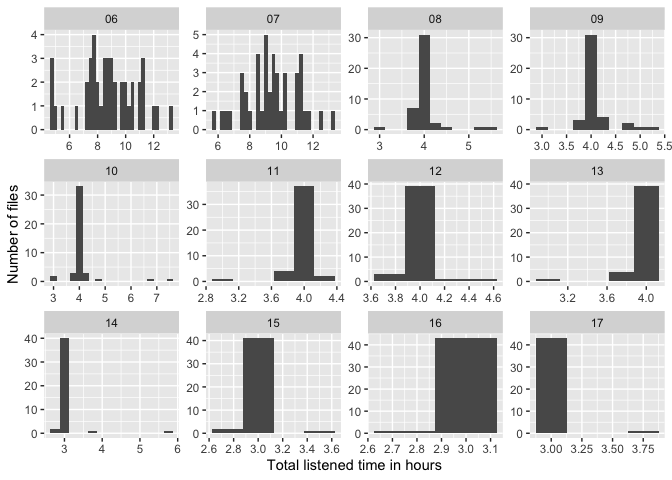
\includegraphics{temp_files/figure-latex/histograms-1.pdf}

\end{document}
